\documentclass[12pt]{article}

% Packages
\usepackage[margin=1in]{geometry}
\usepackage{amsmath,amssymb,amsthm}
\usepackage{enumitem}
\usepackage{hyperref}
\usepackage{xcolor}
\usepackage{import}
\usepackage{xifthen}
\usepackage{pdfpages}
\usepackage{transparent}
\usepackage{listings}
\usepackage{tikz}
\usepackage{physics}
\usepackage{siunitx}
\usepackage{cancel}
  \usetikzlibrary{calc,patterns,arrows.meta,decorations.markings}


\DeclareMathOperator{\Log}{Log}
\DeclareMathOperator{\Arg}{Arg}

\lstset{
    breaklines=true,         % Enable line wrapping
    breakatwhitespace=false, % Wrap lines even if there's no whitespace
    basicstyle=\ttfamily,    % Use monospaced font
    frame=single,            % Add a frame around the code
    columns=fullflexible,    % Better handling of variable-width fonts
}

\newcommand{\incfig}[1]{%
    \def\svgwidth{\columnwidth}
    \import{./Figures/}{#1.pdf_tex}
}
\theoremstyle{definition} % This style uses normal (non-italicized) text
\newtheorem{solution}{Solution}
\newtheorem{proposition}{Proposition}
\newtheorem{problem}{Problem}
\newtheorem{lemma}{Lemma}
\newtheorem{theorem}{Theorem}
\newtheorem{remark}{Remark}
\newtheorem{note}{Note}
\newtheorem{definition}{Definition}
\newtheorem{example}{Example}
\newtheorem{corollary}{Corollary}
\theoremstyle{plain} % Restore the default style for other theorem environments
%

% Theorem-like environments
% Title information
\title{}
\author{Jerich Lee}
\date{\today}

\begin{document}

\maketitle
\begin{solution}
  \textbf{Given data}\\
  \begin{align*}
  n &= 6 \;\text{mol}, &
  T_i &= 300 \;\text{K}, &
  T_f &= 383 \;\text{K}, &
  Q &= 1.45\times 10^{4}\;\text{J}.
  \end{align*}
  
  \textbf{1. Temperature change}\\
  \[
  \Delta T \;=\; T_f - T_i \;=\; 383\ \text{K} - 300\ \text{K} \;=\; 83\ \text{K}.
  \]
  
  \textbf{2. Relate heat input to internal‐energy change}\\
  Under constant volume the heat added equals the change in internal energy:
  \[
  Q \;=\; n\,C_V\,\Delta T.
  \]
  Equipartition gives a molar heat capacity at constant volume
  \[
  C_V \;=\; \frac{f}{2}\,R,
  \]
  where \(f\) is the number of active degrees of freedom and \(R = 8.314\;\text{J\,mol}^{-1}\text{K}^{-1}\).
  
  \textbf{3. Solve for \(f\)}\\
  \[
  f \;=\; \frac{2Q}{n R \Delta T}.
  \]
  
  \textbf{4. Insert numerical values}\\
  \begin{align*}
  f &\,=\, \frac{2\bigl(1.45\times10^{4}\;\text{J}\bigr)}
                 {6\;\text{mol}\,\bigl(8.314\;\text{J\,mol}^{-1}\text{K}^{-1}\bigr)\,(83\;\text{K})} \\[6pt]
    &\,=\, \frac{2.90\times10^{4}\ \text{J}}
                 {4.14\times10^{3}\ \text{J}} \\[6pt]
    &\,\approx\, 7.
  \end{align*}
  
  \textbf{5. Conclusion}\\
  \[
  \boxed{f \;=\; 7\ \text{degrees of freedom}}
  \]
  
  Hence the unknown gas has \(\mathbf{7}\) active degrees of freedom, corresponding to option (b).
  \end{solution}
  \begin{solution}
    \textbf{Given data}\\
    \begin{align*}
    T &= 605\ \text{K}, &
    E_1 &= 3.2\times10^{-20}\ \text{J}, &
    E_2 &= E_1, &
    E_3 &= 4.8\times10^{-20}\ \text{J}.
    \end{align*}
    
    \textbf{1.  Boltzmann factor and partition function}\\
    The Boltzmann factor for a state of energy \(E_i\) is
    \[
    e^{-\beta E_i},\qquad 
    \beta=\frac1{k_B T},\qquad k_B = 1.381\times10^{-23}\ \text{J\,K}^{-1}.
    \]
    
    Compute \(\beta\):
    \[
    \beta = \frac1{(1.381\times10^{-23}\ \text{J\,K}^{-1})(605\ \text{K})}
           \approx 1.20\times10^{20}\ \text{J}^{-1}.
    \]
    
    \textbf{2.  Numerical Boltzmann factors}\\
    \[
    \beta E_1 = (1.20\times10^{20})(3.2\times10^{-20}) \approx 3.83,
    \qquad
    \beta E_3 = (1.20\times10^{20})(4.8\times10^{-20}) \approx 5.75.
    \]
    \[
    e^{-\beta E_1}\approx e^{-3.83}=0.0219,\qquad
    e^{-\beta E_3}\approx e^{-5.75}=0.0032.
    \]
    
    \textbf{3.  Partition function}\\
    Because states 1 and 2 have the same energy and degeneracy 1,
    \[
    Z = e^{-\beta E_1}+e^{-\beta E_2}+e^{-\beta E_3}
      = 2\,e^{-\beta E_1}+e^{-\beta E_3}
      \approx 2(0.0219)+0.0032 = 0.0466.
    \]
    
    \textbf{4.  Probability of being in state 3}\\
    \[
    P_3 = \frac{e^{-\beta E_3}}{Z}
         = \frac{0.0032}{0.0466}
         \approx 0.0686.
    \]
    
    \textbf{5.  Result}\\
    \[
    \boxed{P_3 \approx 0.0685}
    \]
    which corresponds to option (e).
    \end{solution}
    \begin{solution}
      For a system in canonical equilibrium the probability of occupying a state of
      energy \(E_i\) is
      \[
      P_i \;=\; \frac{e^{-\beta E_i}}{Z},
      \qquad
      \beta \;=\; \frac{1}{k_B T},
      \qquad
      Z \;=\; \sum_j e^{-\beta E_j}.
      \]
      
      To have \(P_1 = P_3\) we need
      \[
      e^{-\beta E_1} \;=\; e^{-\beta E_3}.
      \]
      
      \textbf{Case analysis}
      
      \begin{enumerate}
        \item \(\displaystyle T = 0\) (\(\beta \to \infty\)).  
              The Boltzmann factor overwhelmingly favours the \emph{lowest} energy
              state; only that state has non‑zero probability, so \(P_1 \neq P_3\).
      
        \item \(\displaystyle T \to \infty\) (\(\beta \to 0\)).  
              Then \(e^{-\beta E_i} \to 1\) for \emph{all} \(i\):
              every state is equally likely, hence \(P_1 = P_3\).
      
        \item Changing the energies (e.g.\ \(E_2 > E_1\)) does not by itself make
              \(E_1\) equal to \(E_3\), so the probabilities remain unequal unless
              \(T\) is taken to infinity.
      \end{enumerate}
      
      \textbf{Conclusion}
      
      Equal probabilities occur in the high‑temperature limit:
      \[
      \boxed{\;T \to \infty\;} \quad\text{(option (b)).}
      \]
      \end{solution}
      \begin{solution}
        The impurity concentration obeys
        \[
        p \;=\; p_0 \exp\!\left(-\frac{\Delta}{kT}\right)
        \quad\Longrightarrow\quad
        \ln p \;=\; \ln p_0 - \frac{\Delta}{k}\,\frac{1}{T}.
        \]
        
        Hence a graph of \(\ln p\) versus \(x = 1/T\) is a straight line with slope
        \[
        m \;=\; -\frac{\Delta}{k}\;,
        \qquad
        \Delta \;=\; -\,k\,m.
        \]
        The larger the magnitude of the \emph{negative} slope, the larger the energetic
        cost \(\Delta\).
        
        \bigskip
        \textbf{Compute the slopes}
        
        For each material two points \((x_1,y_1)\) and \((x_2,y_2)\) are given.
        Because \(x_1 = 0.5\) and \(x_2 = 2\) for all rows, the denominator
        \(\Delta x = x_2-x_1 = 1.5\) is the same:
        
        \[
        m = \frac{y_2 - y_1}{x_2 - x_1}
            = \frac{y_2 - y_1}{1.5}.
        \]
        
        \begin{center}
        \begin{tabular}{c|c|c|c}
        \textbf{Material} & \(y_1\) & \(y_2\) & \(m = \dfrac{y_2 - y_1}{1.5}\) \\
        \hline
        1 & 28.74 & 25.67 & \(-\,2.05\) \\
        2 & 27.11 & 22.58 & \(-\,3.01\) \\
        3 & 20.71 & 14.71 & \(-\,4.00\) \\
        4 & 29.89 & 29.74 & \(-\,0.10\) \\
        5 & 21.73 & 20.11 & \(-\,1.08\)
        \end{tabular}
        \end{center}
        
        \bigskip
        \textbf{Identify the largest \(\Delta\)}
        
        \[
        \lvert m_3\rvert = 4.00
        \quad>\quad
        \lvert m_2\rvert = 3.01
        \quad>\quad
        \lvert m_1\rvert = 2.05
        \quad>\quad
        \lvert m_5\rvert = 1.08
        \quad>\quad
        \lvert m_4\rvert = 0.10.
        \]
        
        Material \(3\) has the steepest (most negative) slope, so it possesses
        the \emph{largest} energetic cost \(\Delta\).
        
        \[
        \boxed{\text{Material 3}}
        \]
        \end{solution}
        \begin{solution}
          \textbf{Given data}\\
          \begin{align*}
          T_H &= 100^{\circ}\mathrm{C} \;=\; 373\ \mathrm{K}, &
          Q_H &= 1000\ \mathrm{W}, &
          W   &= 600\ \mathrm{W}.
          \end{align*}
          
          \textbf{1. Required efficiency of the engine}\\
          \[
          \eta \;=\; \frac{W}{Q_H}
                 \;=\;\frac{600\ \mathrm{W}}{1000\ \mathrm{W}}
                 \;=\; 0.60.
          \]
          
          \textbf{2. Carnot limit}\\
          The maximum possible efficiency for an engine operating between
          reservoirs at \(T_H\) and \(T_C\) is the Carnot efficiency
          \[
          \eta_{\max} \;=\; 1 - \frac{T_C}{T_H}.
          \]
          Setting \(\eta_{\max} = \eta\) gives the \emph{largest} permissible \(T_C\):
          \[
          0.60 \;=\; 1 - \frac{T_C}{373\ \mathrm{K}}
          \quad\Longrightarrow\quad
          \frac{T_C}{373\ \mathrm{K}} \;=\; 1 - 0.60 = 0.40
          \quad\Longrightarrow\quad
          T_C \;=\; 0.40 \times 373\ \mathrm{K} \;=\; 149.2\ \mathrm{K}.
          \]
          
          \textbf{3. Convert to degrees Celsius}\\
          \[
          T_C\bigl({}^{\circ}\mathrm{C}\bigr)
             \;=\; T_C\bigl(\mathrm{K}\bigr) - 273.15
             \;=\; 149.2 - 273.15
             \;\approx\; -123.95^{\circ}\mathrm{C}.
          \]
          
          \textbf{4. Result}\\
          \[
          \boxed{T_{C,\max} \;\approx\; -124^{\circ}\mathrm{C}}
          \]
          
          Thus the cold reservoir can be no warmer than \(\mathbf{-124^{\circ}\mathrm{C}}\),
          corresponding to option (e).
          \end{solution}
          \begin{solution}
            \textbf{Idea.}  
            At equilibrium the chemical potentials of liquid water (\( \mu_\ell \)) and
            water vapour (\( \mu_g \)) are equal.  For an infinitesimal change that keeps
            the two phases in equilibrium we therefore require
            \[
              d\mu_\ell \;=\; d\mu_g .
            \]
            With the given relation
            \(
              d\mu_X = \dfrac{V_X}{N_X}\,dp - \dfrac{S_X}{N_X}\,dT
            \)
            this becomes
            \[
              \frac{V_g}{N}\,dp - \frac{S_g}{N}\,dT
              \;=\;
              \frac{V_\ell}{N}\,dp - \frac{S_\ell}{N}\,dT ,
            \]
            or
            \[
              (V_g - V_\ell)\,dp \;=\; (S_g - S_\ell)\,dT .
            \]
            
            \medskip
            \textbf{1.\  Simplifications}\\
            For water near its normal boiling point
            \[
              V_g \gg V_\ell ,
            \qquad
              V_g \simeq \frac{RT}{p} \quad (\text{ideal‑gas vapour}),
            \]
            so \(V_g - V_\ell \approx V_g\).
            Hence
            \[
              dp \;=\; \frac{S_g - S_\ell}{V_g}\,dT
                    \;=\; \frac{p\,(S_g - S_\ell)}{RT}\,dT .
            \]
            
            \medskip
            \textbf{2.\  Numerical values}\\
            \begin{align*}
            p &= 1.01300\times10^{5}\;\text{Pa}, &
            T &= 373.15\;\text{K}, &
            R &= 8.314\;\text{J\,mol}^{-1}\text{K}^{-1},\\[6pt]
            \Delta S &= S_g - S_\ell
                     = \left(6.05\times10^{3}\;\frac{\text{J}}{\text{kg\,K}}\right)
                       \bigl(0.018\;\text{kg\,mol}^{-1}\bigr)
                     \approx 1.089\times10^{2}\;\frac{\text{J}}{\text{mol\,K}},\\[6pt]
            dT &= -0.13\;\text{K}\quad(\text{boiling point lowered}).
            \end{align*}
            
            \medskip
            \textbf{3.\  Pressure change}\\
            \begin{align*}
            dp
              &= p\,\frac{\Delta S}{R\,T}\,dT \\[6pt]
              &= \bigl(1.01300\times10^{5}\;\text{Pa}\bigr)
                 \frac{1.089\times10^{2}\;\text{J\,mol}^{-1}\text{K}^{-1}}
                      {8.314\;\text{J\,mol}^{-1}\text{K}^{-1}\;(373.15\;\text{K})}
                 \,\bigl(-0.13\;\text{K}\bigr) \\[8pt]
              &\approx -4.6\times10^{2}\;\text{Pa}.
            \end{align*}
            
            \medskip
            \textbf{4.\  Result}\\
            To lower the boiling point of water by \(0.13\;\text{K}\) the pressure must be
            reduced by
            \[
              \boxed{\lvert\Delta p\rvert \;\approx\; 4.5\times10^{2}\ \text{Pa}} .
            \]
            \end{solution}
            \begin{solution}
              \textbf{Given data}
              \[
              T_0 = 77\;\text{K}, \qquad
              T_h = 294\;\text{K}, \qquad
              W_{\max} = 80\;\text{kJ}=8.0\times10^{4}\ \text{J},
              \qquad
              C = ?\;(\text{assumed constant}).
              \]
              
              \textbf{1. Reversible engine running between a hot reservoir and a cold block}\\
              At any instant the block (cold reservoir) is at temperature \(T_c\) while the
              air (hot reservoir) is fixed at \(T_h\).
              For an infinitesimal heat input \(dQ_h\) from the hot reservoir the Carnot
              engine delivers
              \[
              dW = \Bigl(1-\frac{T_c}{T_h}\Bigr)dQ_h .
              \]
              
              \textbf{2. Relate \(dQ_h\) to the block’s warming}\\
              The heat rejected to the block is
              \(dQ_c = dQ_h - dW = \dfrac{T_c}{T_h}dQ_h\),
              and this heat raises the block’s temperature:
              \[
              dQ_c = C\,dT_c
              \quad\Longrightarrow\quad
              dQ_h = \frac{T_h}{T_c}\,C\,dT_c .
              \]
              
              \textbf{3. Differential work element}\\
              \[
              dW = \Bigl(1-\frac{T_c}{T_h}\Bigr)dQ_h
                  = C\Bigl(\frac{T_h}{T_c}-1\Bigr)dT_c .
              \]
              
              \textbf{4. Integrate from \(T_0\) to \(T_h\)}\\
              \[
              W_{\max}
                = C\int_{T_0}^{T_h}
                      \Bigl(\frac{T_h}{T_c}-1\Bigr)dT_c
                = C\Bigl[T_h\ln\!\Bigl(\frac{T_h}{T_0}\Bigr)
                          - (T_h-T_0)\Bigr].
              \]
              
              \textbf{5. Solve for \(C\)}\\
              \[
              C
                = \frac{W_{\max}}
                       {\,T_h\ln\!\bigl(T_h/T_0\bigr)-(T_h-T_0)} .
              \]
              
              Insert the numbers:
              \[
              \begin{aligned}
              T_h\ln\!\Bigl(\tfrac{T_h}{T_0}\Bigr) &=
                294\,\text{K}\;\ln\!\Bigl(\tfrac{294}{77}\Bigr)
                = 294\times1.339 = 3.94\times10^{2}\,\text{K},\\[4pt]
              T_h-T_0 &= 294-77 = 2.17\times10^{2}\,\text{K},\\[6pt]
              \text{Denominator} &= 3.94\times10^{2}-2.17\times10^{2}
                                 = 1.77\times10^{2}\,\text{K},\\[6pt]
              C &= \frac{8.0\times10^{4}\,\text{J}}{1.77\times10^{2}\,\text{K}}
                 \approx 4.5\times10^{2}\,\text{J\,K}^{-1}.
              \end{aligned}
              \]
              
              \textbf{6. Result}\\
              \[
              \boxed{C \;\approx\; 4.6\times10^{2}\ \text{J\,K}^{-1}}
              \]
              which matches option \(\textbf{(a)}\).
              \end{solution}
              \pagebreak
              \begin{problem}
                \textbf{Practice Question: Frosty Engine}
                
                Suppose that we have a block of metal with \emph{constant but unknown} heat capacity.  
                The block is initially at the temperature of dry ice \((T_0 = 120\;\text{K})\).  
                We use this cold metal block to power a perfectly reversible heat engine, taking the surrounding
                air at room temperature \((T_h = 300\;\text{K})\) as the hot thermal reservoir, and we observe
                that \emph{at most} \(90\;\text{kJ}\) of useful work can be extracted from the engine.
                
                \medskip
                What is the heat capacity of the block?
                
                \begin{enumerate}
                  \item[(a)] \(9.5 \times 10^{2}\;\text{J\,K}^{-1}\)
                  \item[(b)] \(5.1 \times 10^{2}\;\text{J\,K}^{-1}\)
                  \item[(c)] \(2.7 \times 10^{2}\;\text{J\,K}^{-1}\)
                  \item[(d)] \(-4.0 \times 10^{2}\;\text{J\,K}^{-1}\)
                  \item[(e)] \(-1.3 \times 10^{3}\;\text{J\,K}^{-1}\)
                \end{enumerate}
              \end{problem}
              \begin{solution}
                \textbf{Microstates and degeneracies}\\
                \begin{itemize}
                  \item Energy level \(E_1 = 0.4\;\text{eV}\) has degeneracy \(g_1 = 1\).
                  \item Energy level \(E_2 = 0.6\;\text{eV}\) has degeneracy \(g_2 = 2\).
                \end{itemize}
                That gives a total of
                \[
                g_{\text{tot}} \;=\; g_1 + g_2 \;=\; 1 + 2 = 3
                \]
                distinct microstates.
                
                \medskip
                \textbf{Equiprobability at }\(T \to \infty\)\\
                As \(T \to \infty\) every microstate is equally likely, so the probability for
                any single state is
                \[
                P = \frac{1}{g_{\text{tot}}} = \frac{1}{3}.
                \]
                
                \medskip
                \textbf{Average (expectation) energy}\\
                \[
                \langle E \rangle
                  = \sum_{i} P_i E_i
                  = \frac{1}{3}\Bigl(
                      1 \times 0.4\;\text{eV}
                      + 2 \times 0.6\;\text{eV}
                    \Bigr)
                  = \frac{0.4 + 1.2}{3}
                  = 0.533\;\text{eV}.
                \]
                
                \medskip
                \textbf{Result}\\
                \[
                \boxed{\langle E \rangle \approx 0.533\;\text{eV}}
                \]
                
                This corresponds to option \textbf{(d)}.
                \end{solution}
                \pagebreak
                \begin{problem}
                  \textbf{Practice Question: Hot Bath}
                  
                  A system has states with energies \(E_1 = 0.20\;\text{eV}\) and
                  \(E_2 = 0.60\;\text{eV}\).  There is only a single state with energy
                  \(E_1\), but there are \emph{three} states with energy \(E_2\).
                  
                  \medskip
                  What is the average energy of the system as the temperature \(T\) approaches infinity?
                  
                  \begin{enumerate}
                    \item[(a)] \(0.200\;\text{eV}\)
                    \item[(b)] \(0.350\;\text{eV}\)
                    \item[(c)] \(0.500\;\text{eV}\)
                    \item[(d)] \(0.600\;\text{eV}\)
                    \item[(e)] \(0.800\;\text{eV}\)
                  \end{enumerate}
                \end{problem}
                \begin{solution}
                  \textbf{Given data}
                  \[
                  P_i = 700\ \text{Pa},\qquad
                  P_f = 850\ \text{Pa},\qquad
                  T   = 600\ \text{K},\qquad
                  N   = 7.0\times10^{23}\ \text{molecules}.
                  \]
                  
                  \textbf{1.\ Thermodynamic relation at constant \(T\)}  
                  
                  For an ideal gas at fixed temperature the Gibbs free energy changes according to
                  \[
                  dG = V\,dP
                  \quad\Longrightarrow\quad
                  \Delta G = \int_{P_i}^{P_f}\! V\,dP .
                  \]
                  Using the ideal‑gas law \(V = Nk_B T/P\),
                  \[
                  \Delta G = Nk_B T\int_{P_i}^{P_f}\frac{dP}{P}
                           = Nk_B T\ln\!\Bigl(\frac{P_f}{P_i}\Bigr).
                  \]
                  
                  \textbf{2.\ Numerical evaluation}
                  
                  \[
                  \begin{aligned}
                  Nk_B T
                   &= \bigl(7.0\times10^{23}\bigr)\!
                      \bigl(1.380\,649\times10^{-23}\,\text{J K}^{-1}\bigr)
                      (600\ \text{K}) \\[4pt]
                   &= 5.798\times10^{3}\ \text{J},\\[6pt]
                  \ln\!\Bigl(\tfrac{P_f}{P_i}\Bigr)
                   &= \ln\!\Bigl(\tfrac{850}{700}\Bigr)
                   \approx 0.194.
                  \end{aligned}
                  \]
                  
                  \[
                  \Delta G = (5.798\times10^{3}\ \text{J})(0.194)
                           \approx 1.13\times10^{3}\ \text{J}.
                  \]
                  
                  \textbf{3.\ Result}
                  
                  \[
                  \boxed{\Delta G \;\approx\; 1.12\times10^{3}\ \text{J}}
                  \]
                  
                  This corresponds to option \(\mathbf{(c)}\).
                  \end{solution}
                  \begin{align}
                    G &= U - TS + pV
                         \quad\Longrightarrow\quad
                    dG \;=\; dU - T\,dS - S\,dT + p\,dV + V\,dp.  \tag{1}
                    \end{align}
                    
                    \textbf{1.\ Insert the first‑law differential \(dU\).}
                    
                    For a simple compressible system that can exchange particles,  
                    \(dU = T\,dS - p\,dV + \mu\,dN.\)
                    
                    \[
                    dG = (T\,dS - p\,dV + \mu\,dN)\;-\;T\,dS - S\,dT + p\,dV + V\,dp
                        = -S\,dT + V\,dp + \mu\,dN. \tag{2}
                    \]
                    
                    \textbf{2.\ Hold the natural variables of \(G\) fixed.}
                    
                    The natural variables of the Gibbs free energy are \((T,p,N)\), so at **constant temperature** and for a fixed amount of substance,
                    
                    \[
                    dT = 0,\qquad dN = 0
                    \;\Longrightarrow\;
                    dG = V\,dp. \tag{3}
                    \]
                    
                    \textbf{3.\ Integrate between the initial and final pressures.}
                    
                    \[
                    \boxed{\;
                    \Delta G
                      = \int_{P_i}^{P_f} V\,dp
                    \;}
                    \tag{4}
                    \]
                    
                    If the gas is ideal, substitute \(V = \dfrac{Nk_B T}{p}\) (or \(V = \dfrac{nRT}{p}\) per mole) before performing the integral.
                    \begin{solution}
                      \textbf{Background.}
                      The Clausius–Clapeyron relation for the equilibrium vapour pressure of a
                      substance can be written in the empirical form
                      \[
                        p \;=\; p_0 \exp\!\Bigl(-\frac{L}{k_B T}\Bigr),
                      \]
                      where \(L\) is the latent heat \emph{per molecule} (or, if one prefers, use
                      \(L_m = N_A L\) with the molar gas constant \(R\)).  Taking the natural
                      logarithm gives a convenient linearised expression:
                      \[
                        \boxed{\;
                        \ln p = \ln p_0 \;-\;\frac{L}{k_B}\,\frac{1}{T}
                        \;}
                        \tag{1}
                      \]
                      
                      %-------------------------------------------------
                      \subsection*{(i) Sketch of \(\ln p\) versus \(1/T\)}
                      Equation (1) is of the form \(y = b + mx\) with
                      \[
                        y = \ln p,
                        \qquad
                        x = \frac{1}{T},
                        \qquad
                        m = -\frac{L}{k_B}\;(<0),
                        \qquad
                        b = \ln p_0.
                      \]
                      Hence the expected graph is a \emph{straight line with negative slope}.  
                      As \(1/T\) increases (meaning the actual temperature \(T\) decreases),
                      the ordinate \(\ln p\) falls linearly.  The intercept on the ordinate axis
                      (\(1/T = 0\)) is \(\ln p_0\).
                      
                      \begin{center}
                      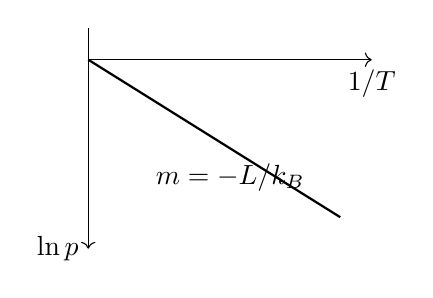
\begin{tikzpicture}[xscale=4, yscale=2]
                        \draw[->] (0,0.2) -- (0,-1.2) node[left] {$\ln p$};
                        \draw[->] (0,0) -- (0.9,0)  node[below] {$1/T$};
                        \draw[thick] (0,0) -- (0.8,-1) node[pos=0.9,above left] {$m=-L/k_B$};
                      \end{tikzpicture}
                      \end{center}
                      
                      %-------------------------------------------------
                      \subsection*{(ii) Extracting \(L\) from the slope}
                      Because the slope of the straight‑line fit to experimental data is
                      \[
                        m = -\,\frac{L}{k_B},
                      \]
                      a measurement of \(m\) immediately yields
                      \[
                        \boxed{\,L = -m\,k_B\,}.
                      \]
                      If the graph is drawn using molar quantities (\(\ln p\) versus \(1/T\) in SI
                      units, but with \(R\) replacing \(k_B\)), then
                      \(
                        L_m = -m\,R
                      \)
                      gives the \emph{molar} latent heat of vaporisation.
                      
                      \medskip
                      \textbf{Practical procedure.}
                      \begin{enumerate}
                        \item Measure the equilibrium vapour pressure \(p(T_i)\) at several
                              temperatures \(T_i\).
                        \item Plot \(\ln p_i\) on the ordinate against \(1/T_i\) on the abscissa.
                        \item Perform a linear regression to obtain the slope \(m\).
                        \item Compute \(L = -m\,k_B\) (or \(L_m = -m\,R\)).
                      \end{enumerate}
                      
                      Because the derivation assumed (i) an ideal gas for the vapour and
                      (ii) a temperature‑independent latent heat over the fitting range,
                      the most accurate \(L\) comes from a reasonably narrow temperature window
                      around the region of interest.
                      \end{solution}
                      \begin{solution}
                        \textbf{Clausius–Clapeyron form used}
                        
                        \[
                        p = p_0 \exp\!\Bigl(-\frac{L}{k_B T}\Bigr)
                        \quad\Longrightarrow\quad
                        \ln\!\frac{p}{p_0} = -\frac{L}{k_B}\Bigl(\frac{1}{T}-\frac{1}{T_0}\Bigr).
                        \]
                        
                        \textbf{Known reference point}
                        
                        \[
                        T_0 = 373\;\text{K}, \qquad p_0 = 1\;\text{atm}.
                        \]
                        
                        \textbf{Latent heat per molecule}
                        
                        The numerical fit in the previous part gave the slope  
                        \(m = -L/k_B \approx -4.89\times10^{3}\),  
                        so
                        
                        \[
                        \frac{k_B}{L} = \frac{1}{|m|} \approx 2.05\times10^{-4}\;\text{K}^{-1}.
                        \]
                        
                        \textbf{Pressure‐cooker condition}
                        
                        \[
                        p = 2\;\text{atm}\quad\Longrightarrow\quad
                        \ln\!\frac{p}{p_0} = \ln 2 = 0.6931.
                        \]
                        
                        \textbf{Solve for the new boiling temperature \(T\)}
                        
                        \[
                        \frac{1}{T}
                          = \frac{1}{T_0} - \frac{k_B}{L}\,\ln 2
                          = \frac{1}{373\;\text{K}} - (2.05\times10^{-4})\,(0.6931).
                        \]
                        
                        \[
                        \frac{1}{T} = 2.680\times10^{-3} - 1.42\times10^{-4}
                                    = 2.538\times10^{-3}\;\text{K}^{-1},
                        \qquad
                        T = \frac{1}{2.538\times10^{-3}}
                          \approx 3.94\times10^{2}\;\text{K}.
                        \]
                        
                        \[
                        \boxed{T \;\approx\; 3.94\times10^{2}\ \text{K} \;\;(121^{\circ}\text{C})}.
                        \]
                        
                        Thus water boils at about \(121^{\circ}\text{C}\) inside a pressure cooker
                        operating at \(2\;\text{atm}\).
                        \end{solution}
                        \begin{solution}
                          At fixed pressure and temperature the Gibbs free energy of a multicomponent
                          system is
                          \[
                          G = \mu_L N_L + \mu_S N_S ,
                          \]
                          where \(\mu_L\) and \(\mu_S\) are the (constant) chemical potentials of the
                          liquid and solid phases, respectively.  
                          A spontaneous transfer of an infinitesimal amount of material \(dN\) from the
                          liquid to the solid changes \(G\) by
                          \[
                          dG \;=\; (\mu_S - \mu_L)\,dN .
                          \]
                          
                          \textbf{Sign of \(\mu_S-\mu_L\).}  
                          The data give
                          \[
                          \mu_L = 5\times10^{-20}\;\text{J}, \qquad
                          \mu_S = 9\times10^{-21}\;\text{J},
                          \]
                          so \(\mu_S < \mu_L\) and therefore \(\mu_S-\mu_L < 0\).
                          
                          \textbf{Direction of spontaneous change.}  
                          Because \(dG < 0\) when \(dN>0\), Gibbs free energy decreases if material is
                          moved \emph{from the liquid to the solid}.  The process will continue until no
                          liquid remains, i.e.\ until \(N_L = 0\).
                          
                          \textbf{Conservation of the total amount of material.}  
                          \[
                          N_{\text{tot}} = N_L + N_S = 5\;\text{mol} + 2\;\text{mol} = 7\;\text{mol}.
                          \]
                          
                          \[
                          \boxed{N_S^{\;\text{eq}} = 7\ \text{mol}}
                          \]
                          
                          \bigskip
                          Hence the equilibrium value of \(N_S\) is \(7\) moles, corresponding to
                          option \textbf{(c)}.
                          \end{solution}
                          \begin{problem}
                            \textbf{Practice Question: Chemical Potential}
                          
                            At a pressure of \(2\ \text{atm}\) and a temperature of \(250\ \text{K}\),
                            a certain substance can exist in two phases: liquid \((L)\) and
                            vapour \((V)\).
                            Initially the system contains
                          
                            \[
                              N_L = 3\ \text{mol}, \qquad N_V = 6\ \text{mol}.
                            \]
                          
                            At these \(P\)–\(T\) conditions the chemical potentials are
                          
                            \[
                              \mu_L = 4 \times 10^{-20}\ \text{J}, \qquad
                              \mu_V = 6 \times 10^{-20}\ \text{J}.
                            \]
                          
                            \medskip
                            What is the equilibrium value of \(N_V\)?
                          
                            \begin{enumerate}
                              \item[(a)] \(0\ \text{mol}\)
                              \item[(b)] \(3\ \text{mol}\)
                              \item[(c)] \(6\ \text{mol}\)
                              \item[(d)] \(9\ \text{mol}\)
                              \item[(e)] \(4.5\ \text{mol}\)
                            \end{enumerate}
                          \end{problem}
                          \begin{solution}
                            \textbf{Equipartition for a crystalline solid}\\
                            At temperatures well above the Debye temperature the Dulong--Petit law
                            applies: each atom contributes \(3k_B\) to the heat capacity at constant
                            volume.  Hence, per \emph{mole},
                            \[
                            C_V^{\text{(molar)}} = 3R,
                            \]
                            where \(R = 8.314\;\text{J\,mol}^{-1}\text{K}^{-1}\).
                            
                            \medskip
                            \textbf{1.\ Convert the mass of germanium to moles}
                            \[
                            M_{\text{Ge}} = 72.63\;\text{g\,mol}^{-1}, 
                            \qquad
                            m = 4.0\;\text{kg} = 4.0\times10^{3}\;\text{g},
                            \]
                            \[
                            n = \frac{m}{M_{\text{Ge}}}
                              = \frac{4.0\times10^{3}\ \text{g}}{72.63\ \text{g\,mol}^{-1}}
                              \approx 55.1\ \text{mol}.
                            \]
                            
                            \medskip
                            \textbf{2.\ Total heat capacity of the block}
                            \[
                            C = n\,C_V^{\text{(molar)}} 
                              = n\,(3R)
                              = 55.1\ \text{mol}\;\times\;3(8.314\;\text{J\,mol}^{-1}\text{K}^{-1})
                              \approx 1.37\times10^{3}\;\text{J\,K}^{-1}.
                            \]
                            
                            \medskip
                            \textbf{3.\ Result}\\
                            \[
                            \boxed{C \;\approx\; 1.37 \times 10^{3}\ \text{J\,K}^{-1}}
                            \]
                            
                            This corresponds to option \textbf{(d)}.
                            \end{solution}
                            \pagebreak
                            \begin{problem}
                              \textbf{Practice Question: Heat Capacity}
                            
                              What is the heat capacity of \(3.0\;\text{kg}\) of solid silicon at room
                              temperature?  Assume that equipartition (Dulong–Petit law) holds
                              and use the molar mass of silicon \(M_{\mathrm{Si}} = 28.09\;\text{g\,mol}^{-1}\).
                            
                              \begin{enumerate}
                                \item[(a)] \(1.2 \times 10^{3}\ \text{J\,K}^{-1}\)
                                \item[(b)] \(2.7 \times 10^{3}\ \text{J\,K}^{-1}\)
                                \item[(c)] \(4.0 \times 10^{2}\ \text{J\,K}^{-1}\)
                                \item[(d)] \(8.7 \times 10^{2}\ \text{J\,K}^{-1}\)
                                \item[(e)] \(3.5 \times 10^{3}\ \text{J\,K}^{-1}\)
                              \end{enumerate}
                            \end{problem}
                            \begin{solution}
                              \textbf{Effective potential in the centrifuge}\\
                              The centrifugal field acts like a uniform gravitational acceleration
                              \(
                              g_{\mathrm{eff}} = 3g = 3(9.8\;\text{m\,s}^{-2}) = 29.4\;\text{m\,s}^{-2}.
                              \)
                              For a dilute gas at thermal equilibrium the number density of molecules of
                              mass \(m\) at height \(h\) obeys the Boltzmann distribution
                              \[
                              n(h) \;\propto\; \exp\!\Bigl[-\frac{m g_{\mathrm{eff}} h}{k_B T}\Bigr].
                              \]
                              Hence the ratio of average populations at two heights \(h_1\) and \(h_2\) is
                              \[
                              \frac{N(h_2)}{N(h_1)}
                                    \;=\;
                                    \exp\!\Bigl[-\,\frac{m g_{\mathrm{eff}}(h_2-h_1)}{k_B T}\Bigr].
                              \]
                              
                              %-------------------------------------------------------------
                              \subsection*{Part 1: Hemoglobin count at \(h_2 = 0.20\;\text{m}\)}
                              
                              \[
                              \begin{aligned}
                              m_{\mathrm{Hb}} &= 1.07\times10^{-22}\;\text{kg},\\
                              h_1 &= 0.03\;\text{m}, \quad
                              h_2 = 0.20\;\text{m}, \quad
                              \Delta h = h_2-h_1 = 0.17\;\text{m},\\
                              T &= 312\;\text{K},\qquad
                              k_B = 1.381\times10^{-23}\;\text{J\,K}^{-1}.
                              \end{aligned}
                              \]
                              
                              Exponent:
                              \[
                              \frac{m_{\mathrm{Hb}}\,g_{\mathrm{eff}}\Delta h}{k_B T}
                              =
                              \frac{(1.07\times10^{-22})(29.4)(0.17)}
                                   {(1.381\times10^{-23})(312)}
                              \approx 0.124.
                              \]
                              
                              Population ratio:
                              \[
                              \frac{N_2}{N_1} = e^{-0.124} \approx 0.883.
                              \]
                              
                              Given \(N_1 = 2.0\times10^{4}\) at \(h_1\),
                              \[
                              N_2 = 0.883\,N_1
                                   \approx 0.883\,(2.0\times10^{4})
                                   \approx 1.77\times10^{4}.
                              \]
                              
                              \[
                              \boxed{N(h_2) \approx 1.77\times10^{4}}
                              \qquad\text{(choice (e)).}
                              \]
                              
                              %-------------------------------------------------------------
                              \subsection*{Part 2: Which molecules dominate at the \emph{top}?}
                              
                              The Boltzmann factor shows that lighter molecules decrease less rapidly with
                              height.  Since
                              \(m_{N_2}=4.65\times10^{-26}\;\text{kg}\ll m_{\mathrm{Hb}}\),
                              nitrogen molecules are far more abundant near the top.
                              
                              \[
                              \boxed{\text{Nitrogen (choice (a)).}}
                              \]
                              \end{solution}
                              \begin{solution}
                                We wish to relate the dilute--solution Boltzmann factor
                                \[
                                  \frac{N_{\mathrm{solute}}}{N_{\mathrm{solvent}}}
                                  \;=\;
                                  C\,e^{-\Delta/k_{B}T}
                                  \tag{1}
                                \]
                                to the familiar vapour‐pressure form
                                \[
                                  p
                                  \;=\;
                                  p_{0}\,e^{-L/k_{B}T},
                                  \qquad
                                  \Longrightarrow\qquad
                                  \ln p
                                  \;=\;
                                  \ln p_{0}-\frac{L}{k_{B}}\frac{1}{T}.
                                  \tag{2}
                                \]
                                
                                \subsection*{1.\  Chemical‐potential equilibrium}
                                For a very dilute ideal solution the chemical potential of component $i$ is
                                \[
                                  \mu_{i}
                                  \;=\;
                                  \mu_{i}^{\circ}(T)+k_{B}T\ln x_{i},
                                \]
                                where $x_{i}$ is the mole (or particle) fraction.
                                At phase equilibrium
                                \(
                                  \mu_{\mathrm{solute}}=\mu_{\mathrm{solvent}}
                                \),
                                so
                                \[
                                  \mu_{\mathrm{solute}}^{\circ}(T)-\mu_{\mathrm{solvent}}^{\circ}(T)
                                  \;=\;
                                  k_{B}T\,
                                  \ln\!\Bigl(\tfrac{x_{\mathrm{solvent}}}{x_{\mathrm{solute}}}\Bigr).
                                \]
                                
                                \subsection*{2.\  Introduce the free‐energy cost}
                                Define
                                \[
                                  \Delta
                                  \;=\;
                                  \mu_{\mathrm{solute}}^{\circ}-\mu_{\mathrm{solvent}}^{\circ}.
                                \]
                                Exponentiation gives
                                \[
                                  \frac{x_{\mathrm{solute}}}{x_{\mathrm{solvent}}}
                                  \;=\;
                                  e^{-\Delta/k_{B}T}.
                                \]
                                
                                \subsection*{3.\  Replace mole fractions by particle numbers}
                                Because the solution is very dilute, the fractions
                                $x_{i}$ are proportional to particle counts $N_{i}$.
                                Any temperature‐independent proportionality factors can be absorbed in
                                a constant $C$, yielding exactly equation~\eqref{1}.
                                
                                \subsection*{4.\  Analogy with vapour pressure}
                                Comparing \eqref{1} with \eqref{2} shows a one‐to‐one correspondence:
                                \[
                                  \begin{array}{c|c}
                                    \text{Dilute solution} & \text{Vapour pressure} \\ \hline
                                    N_{\mathrm{solute}}/N_{\mathrm{solvent}}
                                      & p \\[4pt]
                                    \Delta
                                      & L \\[4pt]
                                    C
                                      & p_{0}
                                  \end{array}
                                \]
                                Both are manifestations of the Boltzmann factor
                                $\exp(-\text{energy}/k_{B}T)$ applied to different physical contexts.
                                \end{solution}
                                \begin{solution}
                                  \textbf{Equipartition for a crystalline solid}  
                                  Above its Debye temperature a solid obeys the Dulong–Petit law, so the
                                  \emph{molar} heat capacity is
                                  \[
                                  C_{V,\mathrm{molar}} \;=\; 3R
                                             \;=\; 3(8.314\;\mathrm{J\,mol^{-1}K^{-1}})
                                             \;=\; 24.94\;\mathrm{J\,mol^{-1}K^{-1}}.
                                  \]
                                  
                                  \textbf{1.\  Experimental (mass‐specific) heat capacity}  
                                  The block absorbs \(Q = 700\;\mathrm{J}\) and its temperature rises by
                                  \(\Delta T = 6\;\mathrm{K}\):
                                  \[
                                  C_{\mathrm{mass}}
                                    = \frac{Q}{m\,\Delta T}
                                    = \frac{700\;\mathrm{J}}{(1.0\;\mathrm{kg})(6\;\mathrm{K})}
                                    = 1.17\times10^{2}\;\mathrm{J\,kg^{-1}K^{-1}}.
                                  \]
                                  
                                  \textbf{2.\  Relate mass‐specific and molar capacities}  
                                  For a substance of molar mass \(M\)
                                  \[
                                  C_{\mathrm{mass}}
                                    = \frac{C_{V,\mathrm{molar}}}{M},
                                  \quad\Longrightarrow\quad
                                  M
                                    = \frac{C_{V,\mathrm{molar}}}{C_{\mathrm{mass}}}.
                                  \]
                                  
                                  \textbf{3.\  Solve for \(M\)}  
                                  \[
                                  M
                                    = \frac{24.94\;\mathrm{J\,mol^{-1}K^{-1}}}
                                           {1.17\times10^{2}\;\mathrm{J\,kg^{-1}K^{-1}}}
                                      = 2.14\times10^{-1}\;\mathrm{kg\,mol^{-1}}
                                      = 2.14\times10^{2}\;\mathrm{g\,mol^{-1}}.
                                  \]
                                  
                                  \textbf{4.\  Result}  
                                  \[
                                  \boxed{M \;\approx\; 214\;\mathrm{g\,mol^{-1}}}
                                  \]
                                  
                                  Hence the correct choice is \textbf{(e)}.
                                  \end{solution}
\end{document}
